\documentclass[11pt,a4paper]{article}
\usepackage[margin=2.2cm]{geometry}
\usepackage{graphicx}
\usepackage{booktabs}
\usepackage{xcolor}
\usepackage{hyperref}
\hypersetup{colorlinks=true,linkcolor=blue!50!black,urlcolor=blue!50!black}
\definecolor{accent}{RGB}{20,70,140}
\setlength{\parskip}{4pt}
\setlength{\parindent}{0pt}
\newcommand{\sect}[1]{\section{\textcolor{accent}{#1}}}

\begin{document}

\begin{center}
{\LARGE\bfseries\textcolor{accent}{UART RTL to GDS Flow}}\\[6pt]
{\large APB3 UART Controller: RTL Design, UVM Verification and SKY130 Physical Design}\\[10pt]
{\bfseries M Kamaraju}\\
\href{https://github.com/MKRAJU-VLSI-HUB/uart-rtl-to-gds-flow}{github.com/MKRAJU-VLSI-HUB/uart-rtl-to-gds-flow}
\quad$\cdot$\quad
\href{https://www.linkedin.com/in/magupallikamaraju/}{linkedin.com/in/magupallikamaraju}
\end{center}

\vspace{4pt}
\begin{center}
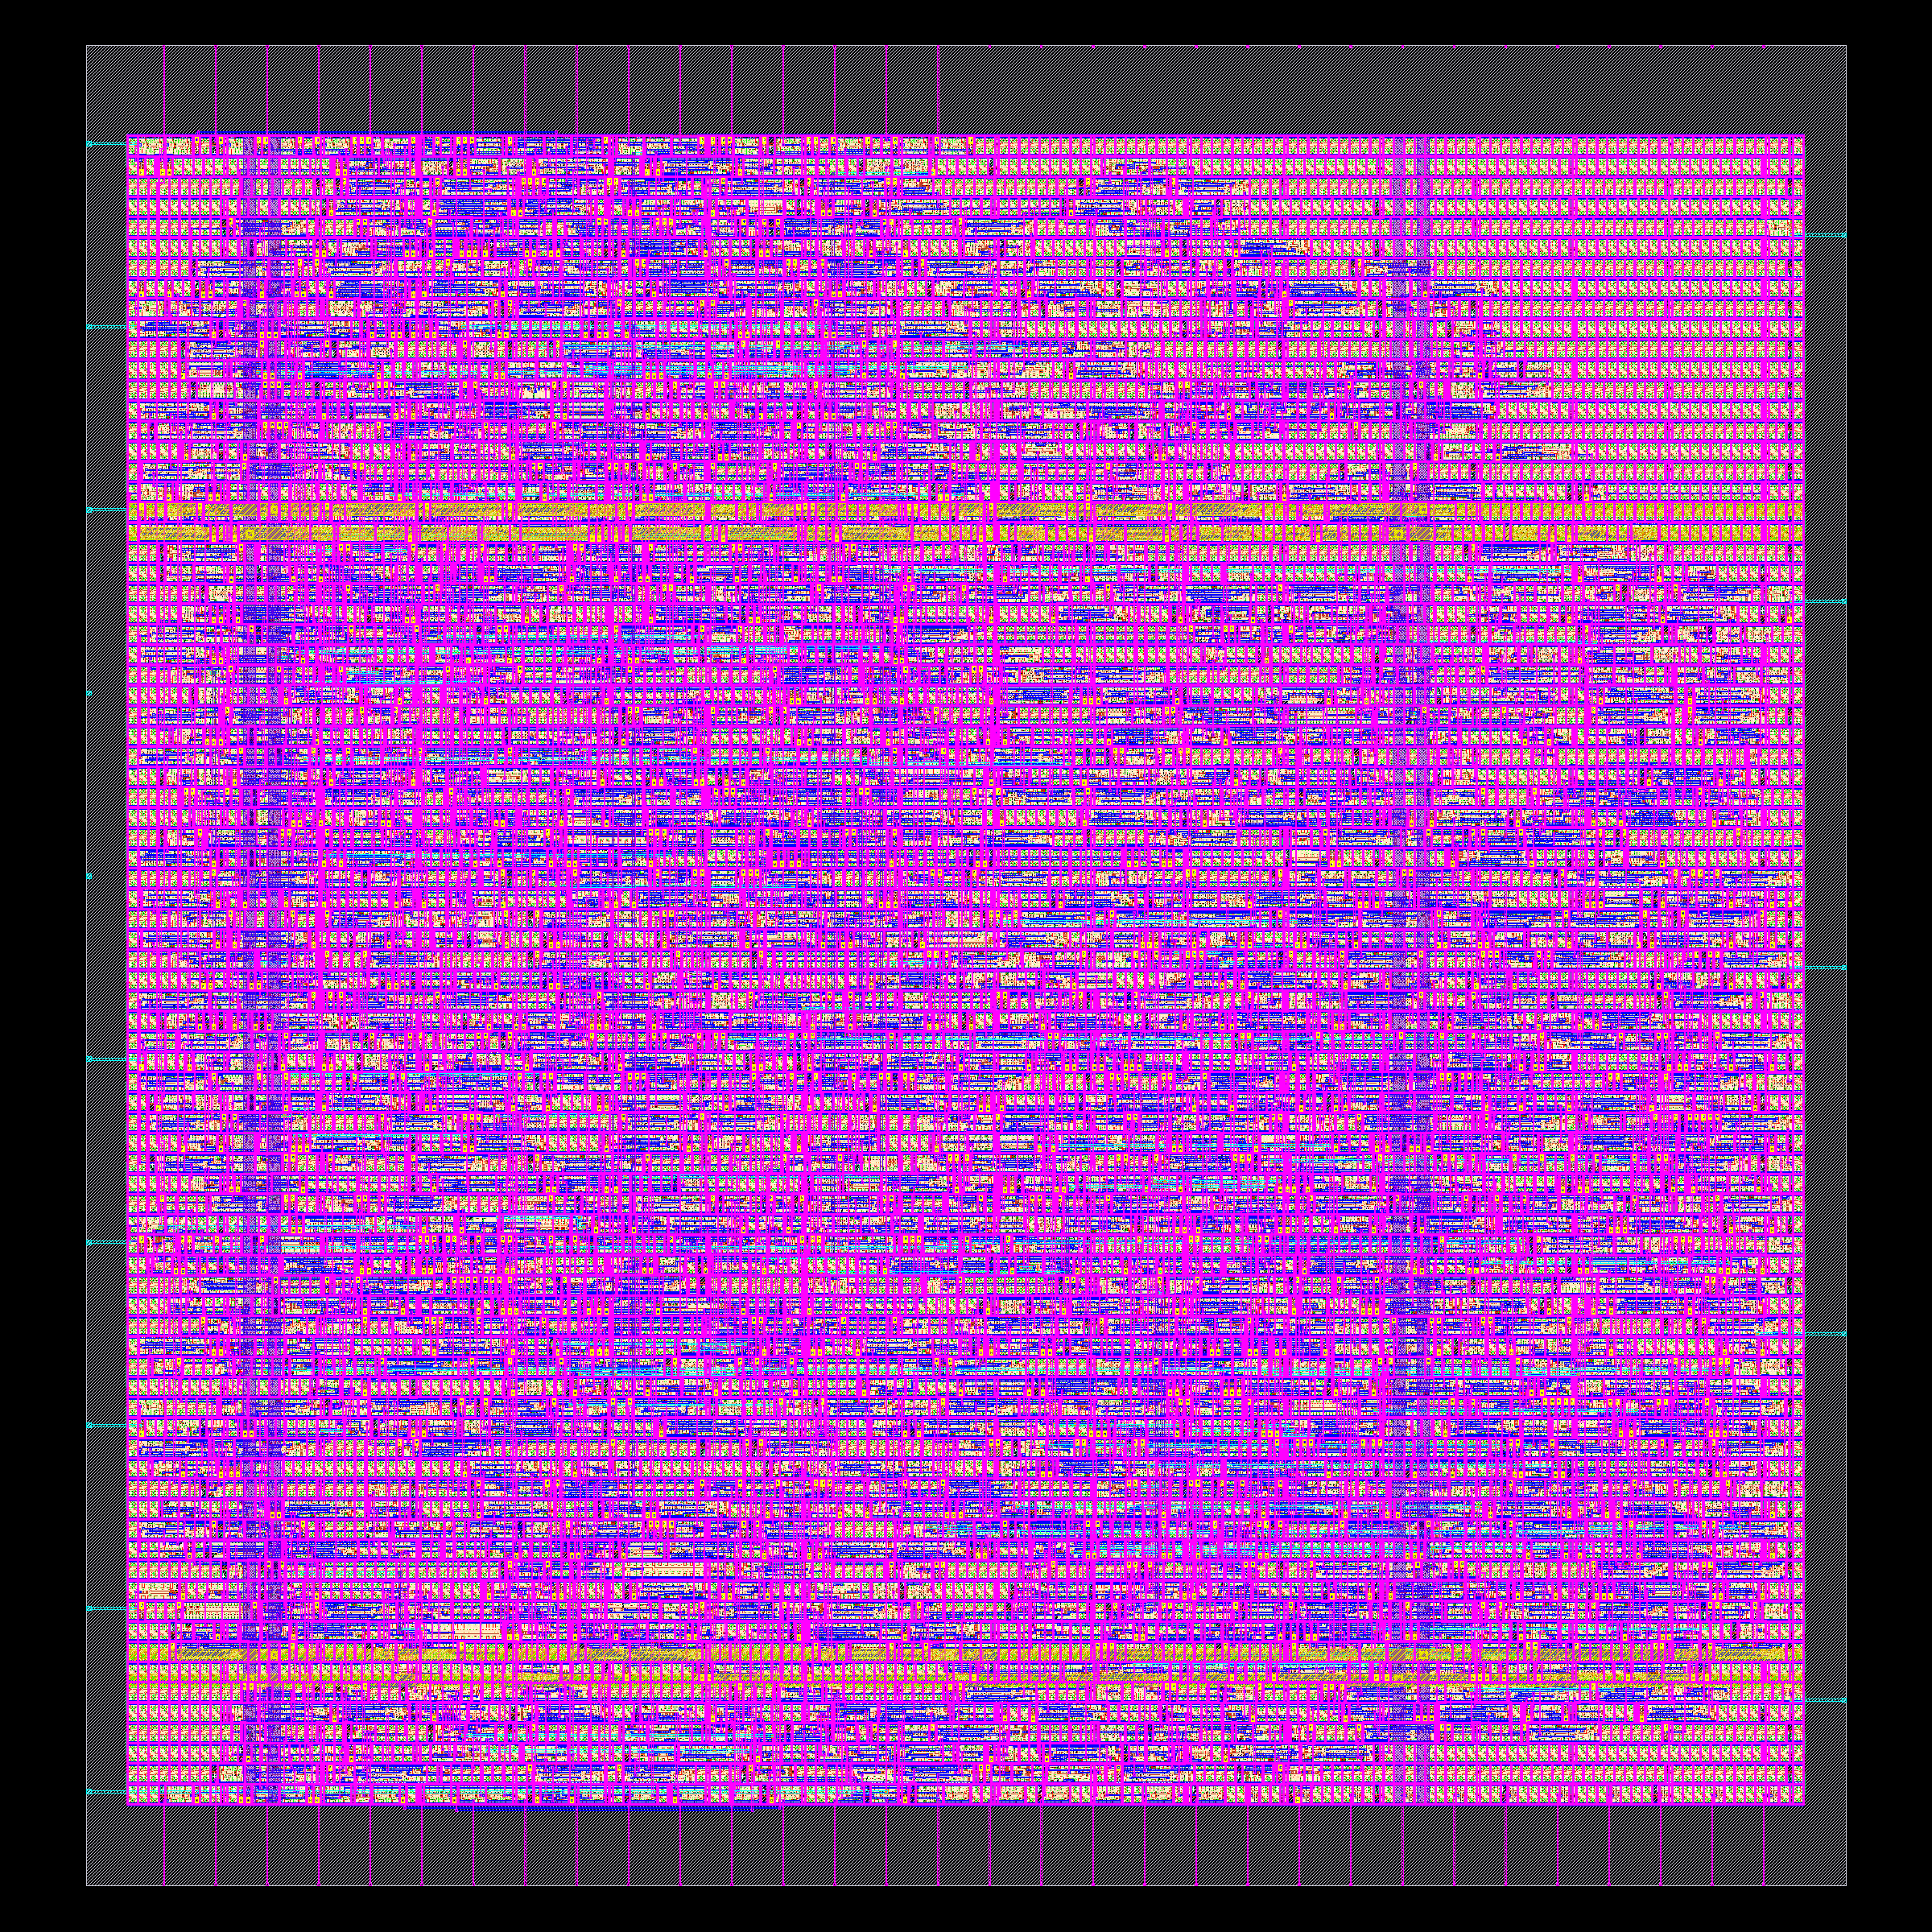
\includegraphics[width=0.62\textwidth]{images/uart_top_layout.png}\\
{\small Final GDSII layout of \texttt{uart\_top} on SkyWater SKY130 (235\,$\mu$m $\times$ 246\,$\mu$m)}
\end{center}

\sect{Project Summary}
This project takes a UART controller with an AMBA APB3 interface through a complete ASIC design flow. The design was written in synthesizable Verilog, verified with a UVM 1.2 environment that uses SystemVerilog assertions and code and functional coverage, and implemented from RTL to GDSII on the open SkyWater 130\,nm PDK using OpenLane~2 (Yosys, OpenROAD, Magic, KLayout, Netgen).

\begin{center}
\begin{tabular}{ll}
\toprule
\textbf{Item} & \textbf{Result} \\
\midrule
UVM regression & 12/12 tests pass, 0 mismatches, 0 assertion failures \\
Functional coverage (merged) & 98.72\,\% \\
Code coverage (DUT) & statement 98--100\,\%, branch 96--100\,\%, condition 93--100\,\% \\
Toggle coverage & 114/114 port and register bits (100\,\%) \\
Signoff frequency & 50\,MHz, met in all 9 PVT/RC corners \\
Setup / hold WNS & +2.22\,ns / +0.11\,ns \\
Die area & 0.058\,mm$^2$ (235.3\,$\mu$m $\times$ 246.0\,$\mu$m) \\
Power (typical) & 2.83\,mW \\
DRC / LVS / antenna & 0 violations / clean / 0 \\
\bottomrule
\end{tabular}
\end{center}

\sect{Design Specification}
\begin{itemize}
\item APB3 slave interface: zero wait state, \texttt{PSLVERR} on unmapped addresses.
\item 16-deep TX and RX FIFOs (first-word fall-through).
\item Programmable baud rate: $f_{baud} = f_{clk} / (16\,(DIV+1))$, with a 16$\times$ oversampling receiver.
\item 5/6/7/8 data bits, none/even/odd parity, 1 or 2 stop bits.
\item Receiver: two-flop synchronizer, mid-bit sampling, start-bit glitch rejection, and re-arming only after the line returns idle (safe on break conditions).
\item Error flags: parity error, framing error, RX overrun, TX overflow (sticky, write-1-to-clear).
\item Six maskable interrupt sources on one \texttt{irq} output, plus an internal loopback mode.
\end{itemize}

\begin{center}
\small
\begin{tabular}{lllp{9.2cm}}
\toprule
\textbf{Off.} & \textbf{Name} & \textbf{Acc.} & \textbf{Description}\\
\midrule
0x00 & TXDATA & W & push byte into TX FIFO \\
0x04 & RXDATA & R & pop byte from RX FIFO \\
0x08 & CTRL & RW & TX\_EN, RX\_EN, PARITY\_EN, PARITY\_ODD, STOP2, DATA\_BITS[1:0], LOOPBACK \\
0x0C & BAUD & RW & 16-bit divisor (reset 26: 115200 baud at 50\,MHz) \\
0x10 & STATUS & R & FIFO full/empty, TX/RX busy, TX and RX FIFO levels \\
0x14 & IER & RW & interrupt enables \\
0x18 & ISR & R/W1C & RX\_AVAIL, TX\_EMPTY, PARITY\_ERR, FRAME\_ERR, RX\_OVERRUN, TX\_OVERFLOW \\
\bottomrule
\end{tabular}
\end{center}

\textbf{RTL hierarchy:} \texttt{uart\_top} contains \texttt{uart\_regs} (APB registers and interrupt logic), \texttt{uart\_baud\_gen} (tick generator), two \texttt{uart\_fifo} instances, \texttt{uart\_tx} (transmit FSM: IDLE, START, DATA, PARITY, STOP, with back-to-back frames) and \texttt{uart\_rx} (receive FSM with oversampling). Frame configuration is latched at the start of every frame, and the serial output is registered so it cannot glitch.

\sect{UVM Verification Environment}
\begin{itemize}
\item \textbf{APB agent:} sequencer, APB3 master driver (setup and access phases, honours PREADY), and monitor.
\item \textbf{UART agent:} a driver that generates frames on \texttt{rxd} with optional parity-error, framing-error and start-glitch injection, plus two monitors that decode frames on \texttt{txd} and \texttt{rxd} using the live configuration.
\item \textbf{Scoreboard / reference model:} TX path (APB writes to frames on \texttt{txd}), RX path (frames on \texttt{rxd} to APB reads), loopback path, TX/RX FIFO occupancy model for overflow and overrun, sticky ISR model with W1C, CTRL/BAUD/IER mirror checks, and PSLVERR decoding.
\item \textbf{Virtual sequences:} reusable APB and UART helpers (program, send, poll, read, drain, duplex) used by 12 tests.
\end{itemize}

\subsection*{Assertions (SVA, bound into the DUT)}
More than 40 concurrent assertions and 10 cover properties check APB protocol rules (PREADY, PENABLE after setup, PSLVERR decoding, known PRDATA), FIFO integrity (count limits, flag consistency, no write when full, no read when empty), single-cycle baud ticks, \texttt{txd} changing only on the bit-tick grid, a start bit after every FIFO pop, idle-high line, RX valid/error pulse qualification, overrun/overflow/parity/framing flag setting, sticky bits cleared only by W1C, \texttt{irq} $=$ OR(ISR \& IER), loopback pin isolation, and reset values.

\subsection*{Regression results (Vivado 2024.2 XSIM)}
\begin{center}
\small
\begin{tabular}{lp{8.3cm}c}
\toprule
\textbf{Test} & \textbf{Scenario} & \textbf{Result}\\
\midrule
uart\_smoke\_test & 8N1 TX and RX & PASS\\
uart\_reg\_test & reset values, R/W patterns, RO registers, PSLVERR & PASS\\
uart\_tx\_test & 16 random formats and baud rates, TX bursts & PASS\\
uart\_rx\_test & 16 random formats, RX with start-bit glitches & PASS\\
uart\_duplex\_test & simultaneous TX and RX & PASS\\
uart\_parity\_err\_test & parity error injection, flag and W1C & PASS\\
uart\_frame\_err\_test & framing error injection, line re-arming & PASS\\
uart\_overrun\_test & 20 frames into a 16-deep RX FIFO & PASS\\
uart\_overflow\_test & 20 writes into a 16-deep TX FIFO & PASS\\
uart\_loopback\_test & internal loopback, random formats & PASS\\
uart\_irq\_test & every interrupt source: set, mask, clear & PASS\\
uart\_random\_test & constrained-random mix of all scenarios & PASS\\
\bottomrule
\end{tabular}
\end{center}

\subsection*{Coverage}
\begin{center}
\small
\begin{tabular}{lr@{\hspace{1.4cm}}lrrr}
\toprule
\textbf{Covergroup} & \textbf{Score} & \textbf{Module} & \textbf{Stmt} & \textbf{Branch} & \textbf{Cond}\\
\midrule
cg\_frame (format cross) & 96.67\,\% & uart\_regs & 100\,\% & 100\,\% & 100\,\% \\
cg\_data & 94.64\,\% & uart\_fifo & 100\,\% & 100\,\% & 92.86\,\% \\
cg\_rx\_err & 100\,\% & uart\_tx & 98.36\,\% & 96.00\,\% & 100\,\% \\
cg\_apb & 98.44\,\% & uart\_rx & 98.59\,\% & 96.30\,\% & 100\,\% \\
cg\_baud, cg\_isr & 100\,\% & uart\_top & -- & 100\,\% & 100\,\% \\
cg\_status, cg\_mode & 100\,\% & & & & \\
\midrule
\textbf{Merged total} & \textbf{98.72\,\%} & \multicolumn{4}{l}{Toggle: 114/114 bits (100\,\%)} \\
\bottomrule
\end{tabular}
\end{center}
The remaining statement and branch holes are the unreachable \texttt{default} arms of the FSM case statements.

\sect{RTL-to-GDSII Implementation (SKY130)}
The flow ran in OpenLane~2: Yosys synthesis, floorplanning with a power distribution network, global and detailed placement, clock tree synthesis, global and detailed routing, RC extraction (min/nom/max), multi-corner static timing analysis, Magic and KLayout DRC, Netgen LVS, and antenna checks. A custom SDC defines a 50\,MHz clock, 30\,\% I/O budgets, clock uncertainty and transition, false paths on the asynchronous reset and the serial input, plus driving cell and load models.

\begin{center}
\small
\begin{tabular}{lr}
\toprule
\textbf{Metric} & \textbf{Value}\\
\midrule
Synthesized cells / flip-flops & 1,398 / 397 \\
Instances after PnR (incl. fill, tap, buffers) & 4,149 \\
Die size & 235.3\,$\mu$m $\times$ 246.0\,$\mu$m \\
Std-cell area / utilization & 29,877\,$\mu$m$^2$ / 59.8\,\% \\
Setup WNS: ss\_100C\_1v60 / tt\_025C\_1v80 / ff\_n40C\_1v95 & +2.34 / +5.00 / +6.03\,ns \\
Worst setup WNS, TNS (9 corners) & +2.22\,ns, 0 \\
Worst hold WNS (9 corners) & +0.11\,ns \\
Clock skew (worst) & 0.28\,ns \\
Total power (typical) & 2.83\,mW \\
Routed wirelength & 59,412\,$\mu$m \\
Magic DRC / KLayout DRC / routing DRC & 0 / 0 / 0 \\
LVS & clean \\
Antenna violations & 0 \\
\bottomrule
\end{tabular}
\end{center}

\textbf{Timing exploration:} with a 100\,MHz target the design met timing in the typical and fast corners (+1.51\,ns setup slack at tt\_025C\_1v80) but missed by 0.64\,ns in the slow corner (ss, 100\,$^\circ$C, 1.60\,V). Signoff was therefore done at 50\,MHz, a typical clock for a UART peripheral, and timing closes with margin in every corner. Some max-slew and max-capacitance warnings remain in the slow-slow corner only.

\begin{center}
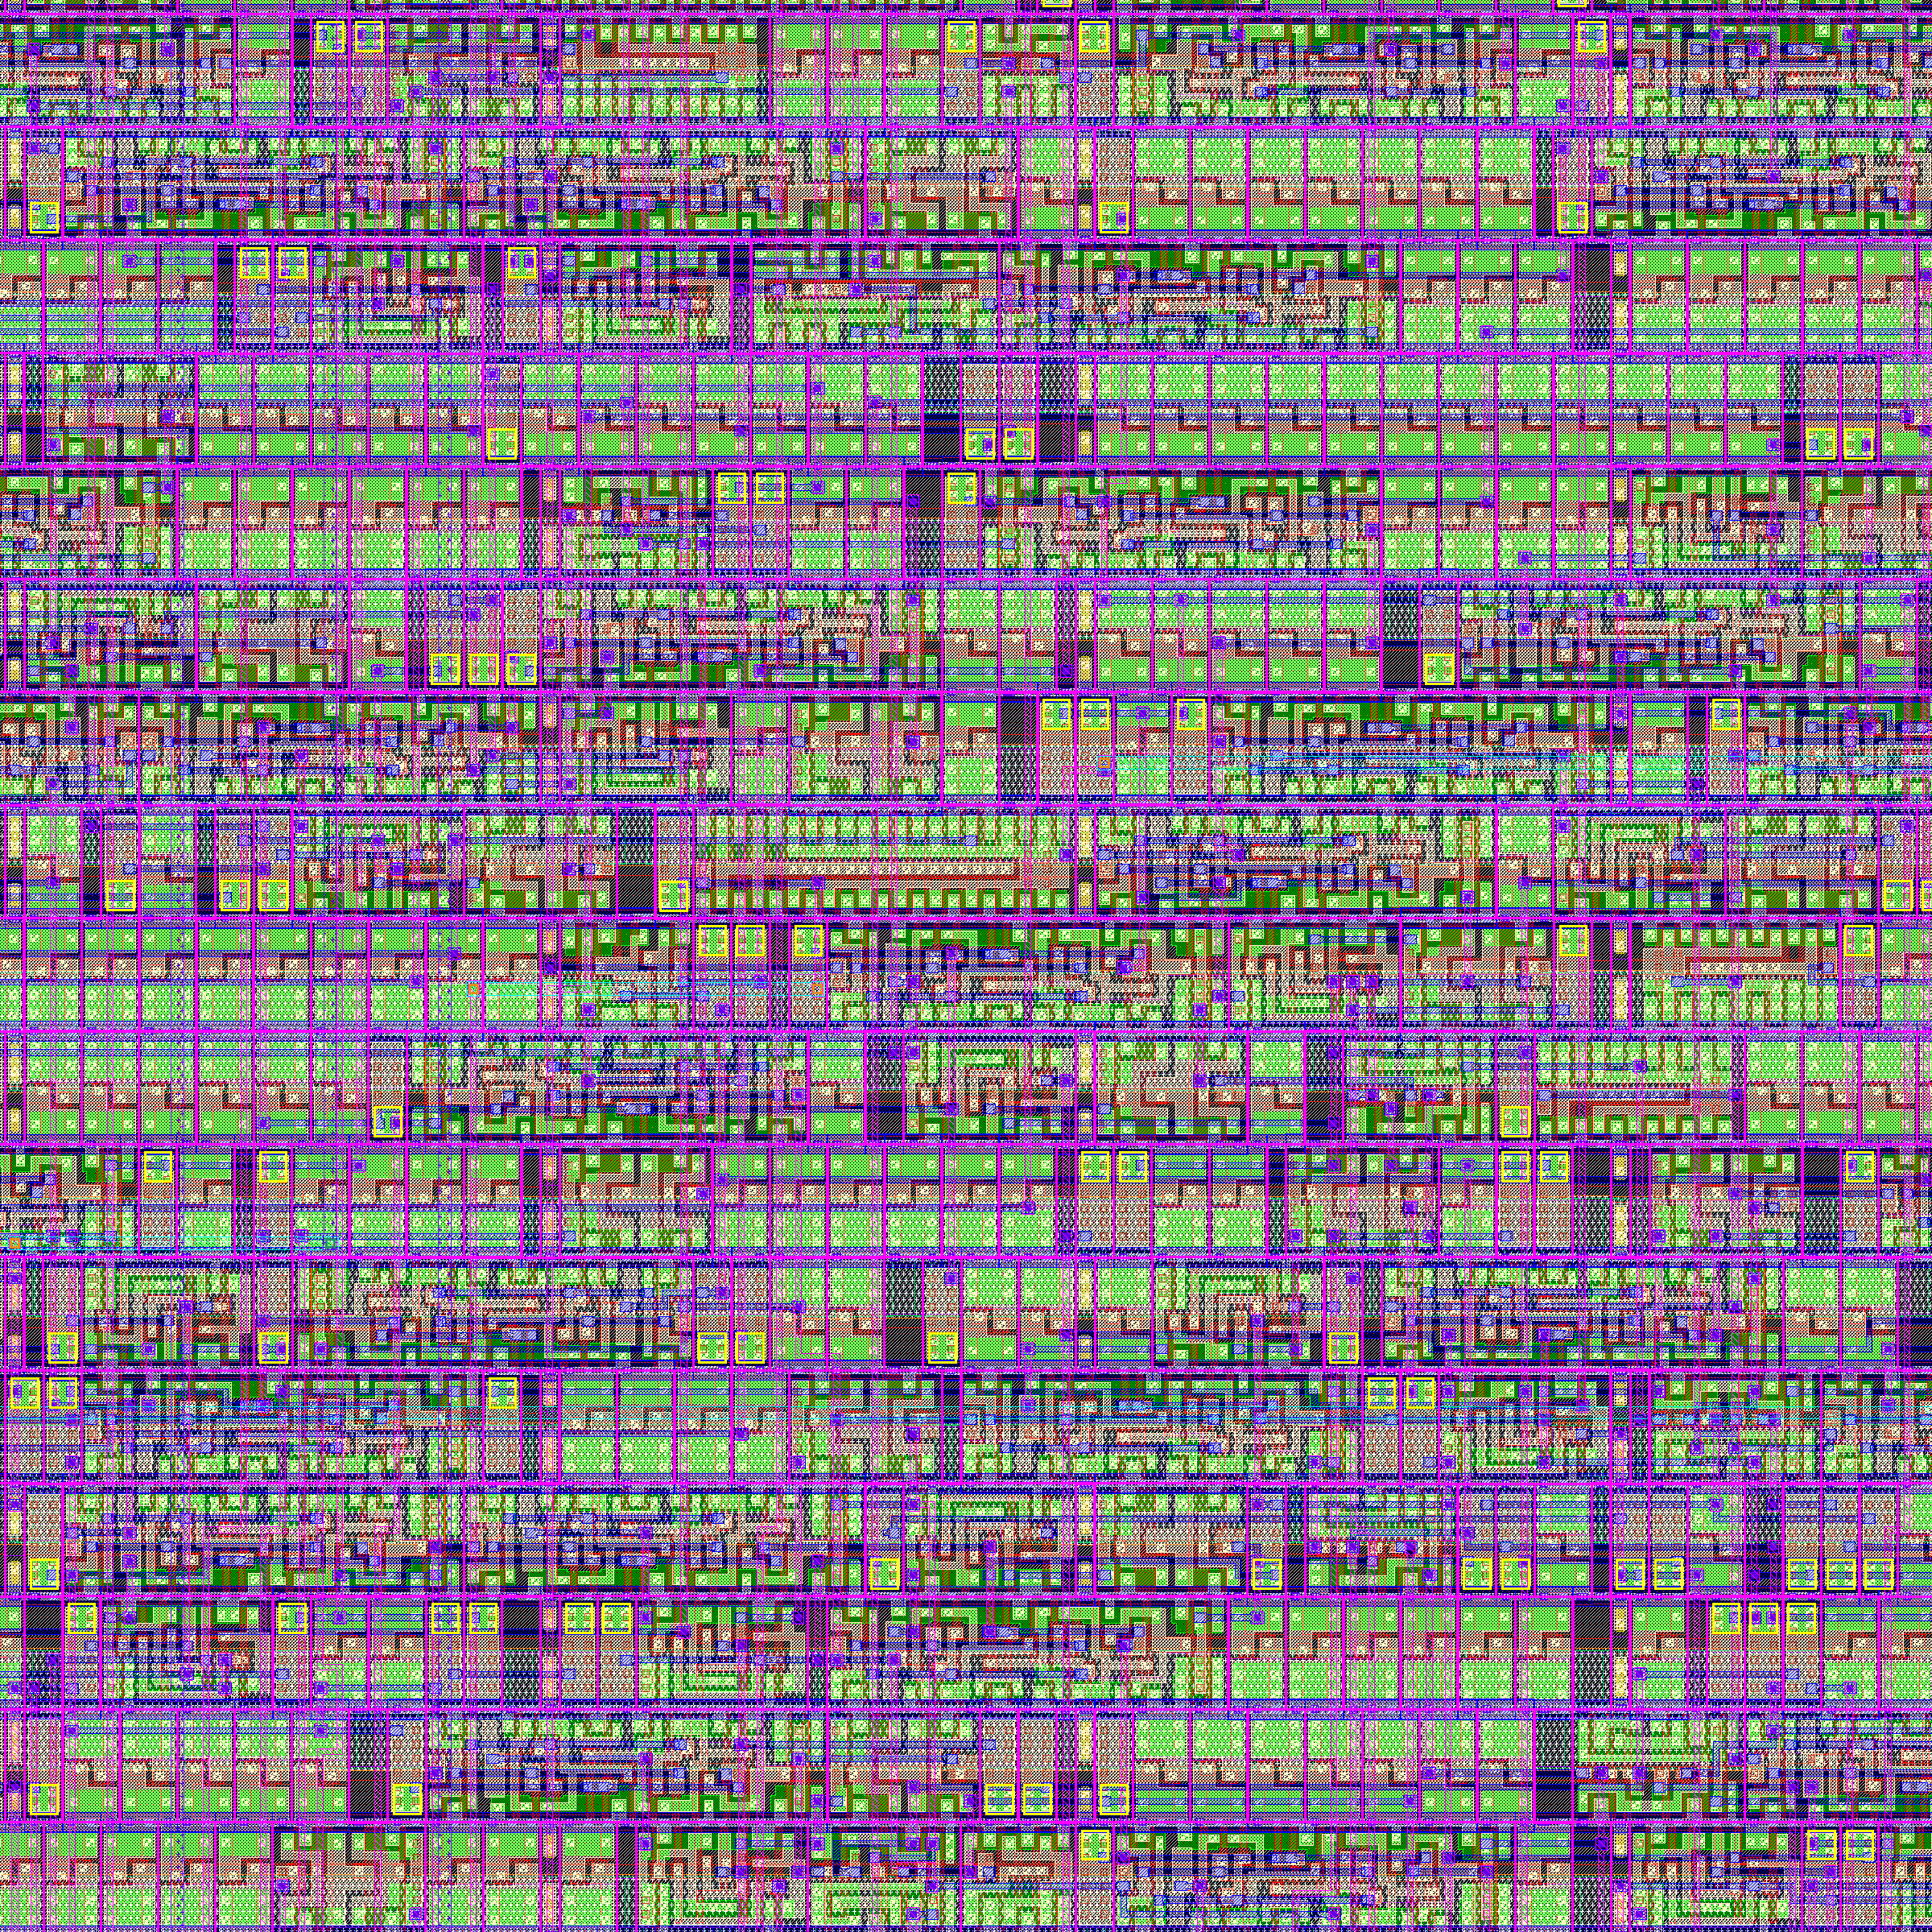
\includegraphics[width=0.48\textwidth]{images/uart_top_layout_zoom.png}\\
{\small Zoomed layout: standard-cell rows, power rails and metal routing}
\end{center}

\sect{Tools}
AMD Vivado 2024.2 XSIM and XCRG (UVM 1.2, SVA, coverage); Yosys; OpenROAD and OpenSTA; Magic; KLayout; Netgen; OpenLane~2 (LibreLane); SkyWater SKY130A PDK (\texttt{sky130\_fd\_sc\_hd}).

\sect{Conclusion}
The APB3 UART was taken from specification to a DRC- and LVS-clean GDSII. Verification closed with a 100\,\% pass rate, 98.7\,\% functional coverage, near-complete code coverage and full toggle coverage, backed by assertion checks. The physical design closes timing at 50\,MHz in all process, voltage, temperature and RC corners in 0.058\,mm$^2$ of SKY130 silicon at 2.83\,mW. All RTL, testbench, scripts, reports and the final GDS are available in the GitHub repository.

\end{document}
